\chapter{Implementierung}\label{chapter_5}
Die praktische Umsetzung des Entwurfs vom vorigen Abschnitt wird in diesem Kapitel beschrieben. Die Implementierung hat das Ziel die Umsetzung der zuvor entworfenen Ansichten, sowie die Realisierung der Anwendung auf der Zielplattform. Im folgenden wird die Architektur und der Aufbau beschrieben. Anschließend werden die wichtigsten Entscheidungen, die bei der Implementierung getroffen wurden erklärt.

\section{Anwendungsarchitektur}
Damit die Entwicklung der Anwendung beschleunigt werden kann, indem wiederverwendbare Muster in der Anwendung verwendet werden, wird zuerst eine geeignete Anwendungsarchitektur benötigt. Als erste Voraussetzung muss diese von der Zielumgebung, bzw. von der Technologie unterstützt werden. \par 

Aufgrund des Offline-Modus in der Anwendung, sowie die Verwendung des Konfigurationsservers müssen zwei unterschiedliche Formen der Datenanbindung unterstützt werden. Dies hat zur Folge, dass ein einfacher Austausch der Datenanbindung in der Anwendung möglich sein muss, ohne eine Neuimplementierung der Schnittstellen. Die Anforderung an ein ästhetisches Design kann durch eine klare Trennung der Ansicht mit den Logikkomponenten erfüllt werden. Damit ist es möglich, die Gestaltung frei von der notwendigen Logik umzusetzen und sich auf das Aussehen der Benutzerschnittstelle zu konzentrieren. Die Architektur muss ebenfalls für Erweiterungen offen sein, damit bei zusätzlichen Anforderungen, die beim Einsatz der Anwendung entstehen, eine Umsetzung folgen kann.

\subsection{MVVM}
Eine Lösung für die oben genannten Anforderungen an die Architektur bietet das von Microsoft entwickelte Model-View-ViewModel (MVVM) Entwurfsmuster. Hier wird eine strikte Trennung zwischen der Ansicht (View), der Logik (ViewModel) und den Daten (Model) vorgenommen. \par 

\begin{figure}
\centering
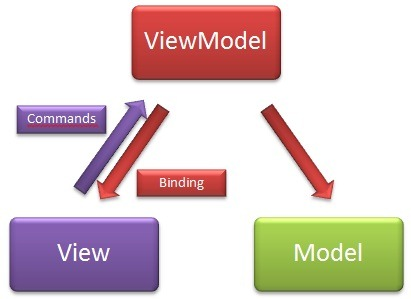
\includegraphics{images/mvvm}
\caption{Komponenten im MVVM Entwurfsmuster}
\label{mvvm}
\end{figure}
Die Kommunikation der einzelnen Komponenten ist in Abbildung \ref{mvvm} dargestellt. Die unterste Ebene ist die Model-Schicht. Diese ist für das Bereitstellen und Persistieren der Daten zuständig. Dies wird entweder mit einer Datenbank oder Webserviceschnittstelle realisiert. Wichtig bei dieser Schicht, wie in der Abbildung zu sehen, ist die unidirektionale Verbindung mit dem ViewModel. Da dies die einzige Verbindung zum Model ist, wird eine Manipulation von weiteren Komponenten verhindert. Dies vereinfacht das Finden von Fehlern, da es nur eine Schnittstelle gibt, die eine Veränderung der Daten durchführt. \par
Auf der anderen Seite ist die View. Diese Komponente ist für das Darstellen der Daten zuständig. Es werden alle Komponenten einer Benutzerschnittstelle auf dieser Ebene verwendet. Der Benutzer führt alle Interaktionen mit dem Programm mit einem Eingabegerät wie der Maus oder Tastatur auf dieser Anwendungsschicht durch. Die Auswertung der Benutzereingaben folgt im "'Modell der Ansicht"' \cite[S.9]{bib:mvvm}, dem ViewModel. Hier werden die Eingaben behandelt und die entsprechenden Aktionen ausgeführt. Diese Schicht ist der Vermittler zwischen den Daten und der Benutzerschnittstelle. Aus diesem Grund werden die Daten, die vom Model erhalten werden für die Ansicht aufbereitet. Die Verbindung zur View-Ebene ist dabei bidirektional, damit sowohl Benutzereingaben, sowie Veränderungen im ViewModel registriert werden. Die Besonderheit liegt hier an der "'losen"' Bindung. Diese sorgt dafür, dass die Anwendung nicht abstürzt, wenn ein bestimmtes Element nicht vorhanden ist, was von der View erwartet wird. 
\par 
Die Anforderung für einen einfachen Austausch der Datenquelle wird durch die Unabhängigkeit des Models erfüllt. Hierdurch können die Daten sowohl auf dem Gerät, als auch mit Webserviceschnittstellen geladen werden. Das MVVM Entwurfsmuster wird von der Technologie unterstützt und es sind bereits Codebeispiele vorhanden \cite{bib:winMvvm}. Mit der Trennung von View und ViewModel ist ein einfaches Erstellen von Benutzerschnittstellen möglich. Aufgrund der Unabhängigkeit beider Komponenten können diese auch separat entwickelt werden. Hierdurch wird es beispielsweise möglich, dass ein Designer und ein Programmierer unabhängig voneinander arbeiten können. 

\subsection{Anwenden des Entwurfsmusters}
Bei der Implementierung der Anwendung mussten für die Anzeige der Daten immer wiederkehrende Eigenschaften der Datensätze verwendet werden. Ein Beispiel für eine solche Eigenschaft ist der Name oder die Beschreibung eines Flugzeuges oder Upgrades. Da beim MVVM Entwurfsmuster die View nicht auf das Model zugreift, kennt es diese Datenobjekte nicht. Aus diesem Grund muss das ViewModel diese Daten konvertieren und ein neues Objekt bereitstellen. 

Ebenfalls muss bei einer Manipulation oder Auswahl der Daten die Konvertierung rückgängig gemacht werden, damit das Model die Änderungen vornehmen kann. Diese Vorgehensweise hat bei einer Veränderung der Daten zur Laufzeit Vorteile, da das ViewModel den Zeitpunkt der Persistierung entscheiden kann und damit evtl. ein Rückgängig anbieten kann. Im Anwendungsbeispiel ist dies jedoch ein zusätzlicher Aufwand, der nicht benötigt wird, da keine Daten manipuliert werden, sondern lediglich eine Auswahl getätigt wird. Die eigentliche Datenbasis wird in der Anwendung nicht verändert.
Für die Vermeidung des zusätzlichen Aufwandes wurde eine neue Komponente eingeführt. Auf diese haben alle drei Ebenen im MVVM Zugriff. In dieser Komponente sind die festen Datenelemente definiert. Es wird nur ein lesender Datenzugriff ermöglicht. Die konkrete Implementierung der Datensätze wird weiterhin im Model vorgenommen. Damit muss keine Konvertierung der Daten erfolgen, um der View einen Zugriff auf die Daten zu geben. \par 
\begin{figure}
\centering
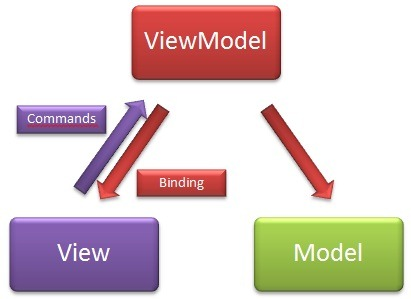
\includegraphics{images/mvvm}
\caption{Klassendiagramm im MVVM Entwurfsmuster}
\label{mvvmApp}
\end{figure}
Die einzelnen Objekte der Anwendung sind in der Abbildung \ref{mvvmApp} zu sehen. In der View Schicht sind die sogenannten Pages enthalten. Eine Page ist die Oberflächenschnittstelle im Windows 8 Framework.  Diese beinhaltet XML Elemente, sogenannten XAML Code. Mit diesem wird deklarativ eine Benutzerschnittstelle erstellt. Für jede, in Kapitel \ref{chapter_4} entworfene Ansicht ist eine Page vorhanden. Für jede Ansicht existiert ein passendes ViewModel, welches Programmcode für die Behandlung der Benutzereingaben enthält. Die Daten werden aus dem Model

Dazu gehört jeweils ein eigenes ViewModel.  Diese verwenden auch mehrfach die Basis Model Komponenten. Die konkreten Datenelemente werden in der Model-Schicht implementiert. 


\section{Navigation}
\section{Expertenmodus}
\section{Anpassungen an die Zusammenfassung}
